\section{Data Collection}
\label{sec:label}


In this section, we discuss how we collect and preprocess data from VirusTotal. 

\begin{figure}[t!]
\begin{center}
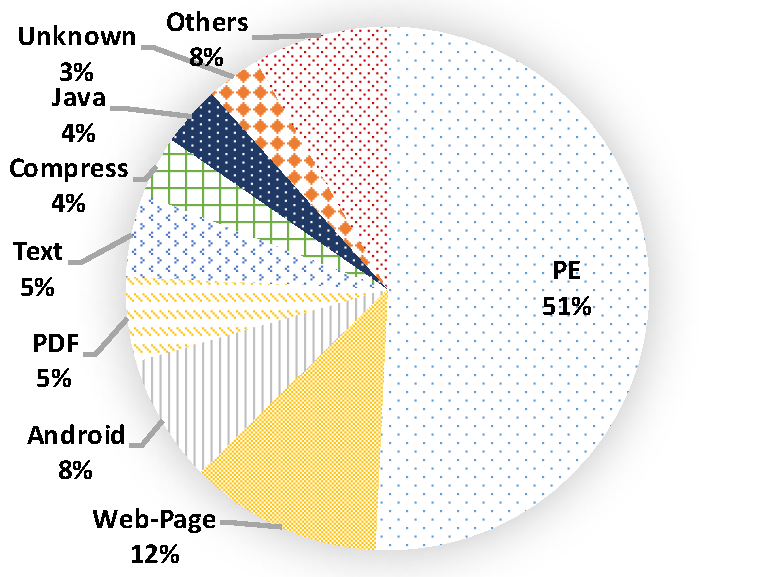
\includegraphics[width=2.5in]{figure/type}
\mycaption{fig:type}{File types for all submissions.}
{
File types and their distributions for all VirusTotal submissions from 2016/05/07 to 2016/09/06. 
}
\end{center}
%\vspace{-0.25in}
\end{figure}



\begin{table}[h!]
\centering
\footnotesize
{
%\begin{tabular}{@{\hspace{3pt}}l@{\hspace{3pt}}|@{\hspace{3pt}}c@{\hspace{3pt}}}
\begin{tabular}{l|l}
\hline
Metadata Field & Explanation \\
\hline                            
%\cline{1-1}
{\bf name}      & submitted file name \\
{\bf link}      & where to download the file \\
{\bf timestamp} & timestamp when the submission was made \\
{\bf source\_country} & the country where the submission was made \\
{\bf source\_id} & user ID making the submission\\
{\bf size} & file size \\
{\bf type} & file type \\
{\bf tags} & labels with more specific information for each {\bf type}\\
{\bf first\_seen} & when the same file was first submitted \\
{\bf last\_seen} & when the same file was last submitted \\
{\bf hashes} & sha1, sha256, md5, and vhash\\
{\bf ssdeep} & ssdeep information digest string \\
{\bf total} & number of engines analyzing the file \\
{\bf positives} & number of engines that flagged the file as malicious \\
{\bf positives\_delta} & changes in {\bf positives} across different submissions\\
{\bf report} & detailed detection report from each AV engine \\
%\multicolumn{2}{|l|}
\hline

\end{tabular}
}
\mycaption{tab:fields}{VirusTotal Metadata.}
{ 
Fields for each submission retrieved from the VirusTotal distribution API and their relation explanation.
The same file can be submitted multiple times by different users.
}
%\vspace{-0.1in}
\end{table}




We collect metadata for each submission through VirusTotal’s distribution API. 
Distribution API keeps returning metadata for latest files submitted to VirusTotal.
Table~\ref{tab:fields} shows the metadata fields and their meaning.  
We began our data collection on May 7th 2016, 
and ended our data collection on September 6th 2016. 
We insert all collected metadata into a cassandra table by using the combination of sha256, source\_id, and timestamp as key.
In total, we collect metadata for 151 million submissions. 

Figure~\ref{fig:type} shows the file type distribution for all submissions. 
Among all file types, \textit{Portable Executable} (PE) files have the largest number, which is the same as results from a previous study~\cite{SongAPsys2016}.
PE files occupy 51\% of all submissions. 
Web pages and malwares on Android have the second and third largest number of malwares, 
occupying 12\% and 8\% of all submissions respectively. 
Other popular file types include PDF, Text, compressed files, and Java files, which is slightly different from the previous study~\cite{SongAPsys2016}. 

Similar to the previous study~\cite{SongAPsys2016}, 
we focus our study in this paper on PE files, 
and leave studies on other types of malwares in the future. 
If the type field for a submission is either ``Win32EXE'' or ``Win32DLL'', 
we consider the submission is a PE file. 
In total, we collect 76 million PE submissions. 
The number of submissions and the number of PE submissions we collected each day are shown in Figure~\ref{fig:subnum}. 

\begin{figure}[t!]
\begin{center}
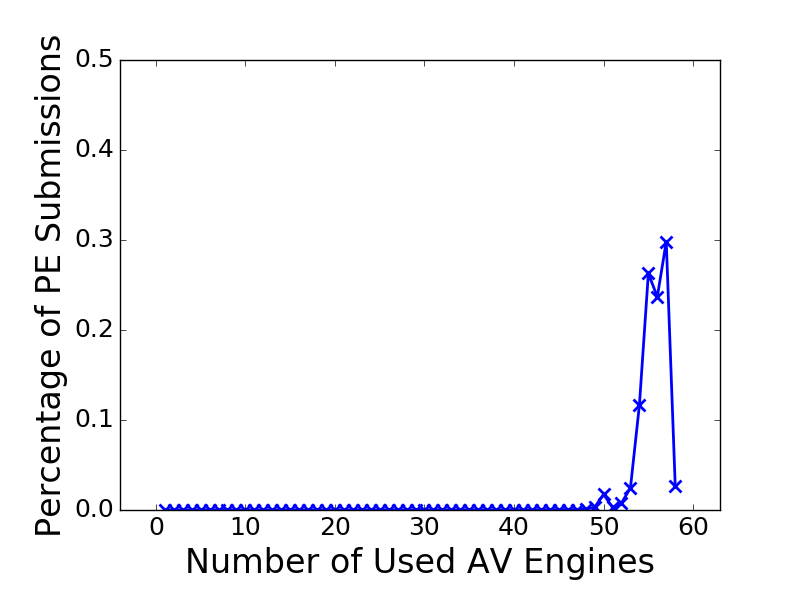
\includegraphics[width=2.5in]{figure/numVendor}
\mycaption{fig:vendornum}{The distribution for the number of used anti-virus engines.}
{
How the number of used anti-virus engines distributes among all PE submissions we collect.
}
\end{center}
%\vspace{-0.25in}
\end{figure}

\begin{figure}[t!]
\begin{center}
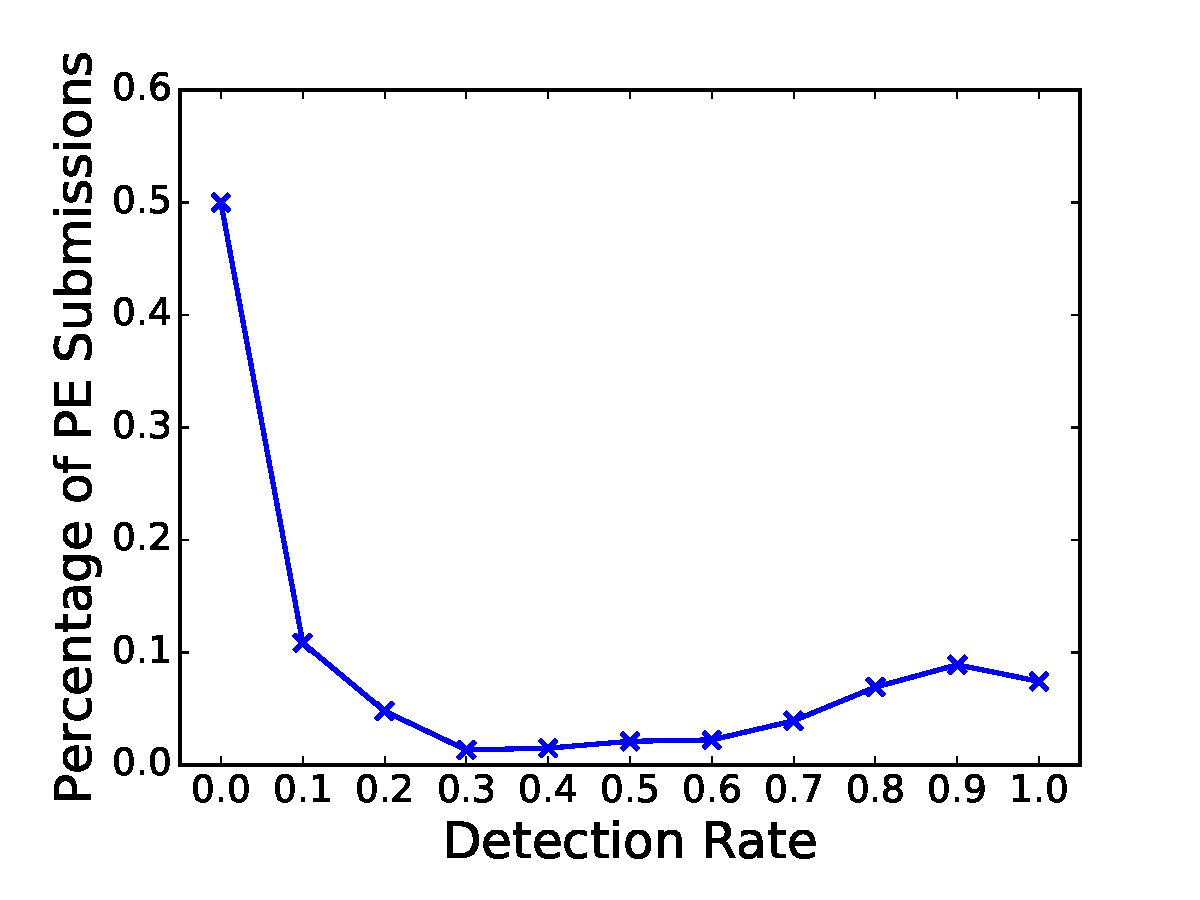
\includegraphics[width=2.5in]{figure/DetectionRate}
\mycaption{fig:detectiorate}{The distribution for detection rate.}
{
How detection rate distributes among all PE submissions we collect.
}
\end{center}
%\vspace{-0.25in}
\end{figure}

For each PE submission, VirusTotal will use a bunch of anti-virus engines to analyze it.
As shown in Table~\ref{tab:fields}, 
total field is to represent the number of used anti-virus engines. 
Figure~\ref{fig:vendornum} shows the distribution for the number of used anti-virus engines. 
More than 99\% of PE submissions are analyzed by at least 50 anti-virus engines. 
Some anti-virus engines will identify a submitted PE file as malware, while others will not. 
Positives field in Table~\ref{tab:fields} represents the number of anti-virus engines identifying the submission as malwares. 
%We calculate detection rate for a submission by using total number to divide positives number. 
%Figure~\ref{fig:detectiorate} shows how detection rate distributes among all PE submissions. 

$$ \textrm{\textit{Detection Rate}} = \dfrac{positives}{total + 1}$$

Detection rate represents the percentage of engines identifying the submission as malware. 
Adding one to total is to avoid dividing 0 exception, and more importantly, 
to give submissions identified by more engines higher detection rate. 
For example, after adding one, submissions analyzed by 50 engines and detected by 50 engines will have a higher detection rate 
than submissions analyzed by 1 engine and detected by 1 engine. 
This formula shares the same intuition from previous work~\cite{GuoICSE2010}, when computing reputations for bug reporters. 
A larger detection rate means more malicious of the malware. 
Figure~\ref{fig:detectiorate} shows how detection rate distributes among all PE submissions. 


One PE file could be submitted more than once to VirusTotal. 
There are 6.72\% PE files submitted more than once to VirusTotal. 
On average, each PE file is submitted 1.19 times. 
Some anti-virus engines may change their results when analyzing the same file during different submissions.
We will discuss how vendors influence each other and how to predict possible detection result change in Section~\ref{sec:influ}.

Like all other empirical study works, 
our findings and conclusions need to be considered with our methodology in mind. 
We use distribution API to download submissions' metadata from VirusTotal. 
There is no guarantee that all data can be successfully downloaded. 
It could be possible that some files are submitted to VirusTotal, 
but we fail to get their information from VirusTotal.
Although we have collected huge amount of malware information from VirusTotal,
we do believe that there are malwares never submitted to VirusTotal, 
or submitted to VirusTotal much later than they appear in the real world. 
However, there are no conceivable ways to study them.
We believe the 4-month malware information we collect can serve as a representative sample for malwares in the real world. 
